\documentclass[a4paper,journal]{IEEEtran}
\usepackage{hyperref}
\usepackage{physics}
\usepackage{amsmath,amsfonts}
\usepackage{algorithmic}
\usepackage{array}
\usepackage[caption=false,font=normalsize,labelfont=sf,textfont=sf]{subfig}
\usepackage{textcomp}
\usepackage{stfloats}
\usepackage{url}
\usepackage{verbatim}
\usepackage{graphicx}
\graphicspath{{./pictures/}}
\usepackage{physics}
\usepackage{balance}
\usepackage{enumitem}

\hyphenation{op-tical net-works semi-conduc-tor IEEE-Xplore}
\usepackage{balance}

%\usepackage[backend=biber]{biblatex}
\bibliographystyle{IEEEtran}

\usepackage[ngerman]{babel}
\DeclareMathOperator{\Landau}{\mathcal{O}} % Landau/Big-O Notation
\DeclareMathOperator{\fraction}{fraction}
\DeclareMathOperator{\eqq}{\widehat{=}}


\begin{document}

\begin{abstract}
  Seit der Entwicklung des theoretischen Konzepts eines Quantencomputers in den 1980er Jahren
  wurden Quantenalgorithmen entworfen,
  die durch die Ausnutzung der Quantenmechanik bestimmte Berechnungen effizienter lösen können
  als die schnellsten bekannten klassischen Algorithmen.
  Insbesondere betreffen sie mathematische Probleme,
  die die Grundlage aktueller kryptografischer Verfahren bilden.
  Obwohl derzeit keine Quantencomputer mit ausreichender Rechenleistung existieren,
  hat die Entwicklung in den letzten Jahren an Geschwindigkeit gewonnen und
  sollte aufgrund der erwarteten zukünftigen Fortschritte in der IT-Sicherheit berücksichtigt werden.

  Um eine Grundlage für die zukünftige Anwendung von Quantenalgorithmen zu schaffen,
  wird eine eigene Bibliothek mit den bekanntesten Quantenalgorithmen entwickelt.
  Die Implementierungen umfassen ressourcensparende Varianten,
  die gleichzeitig skalierbar sind,
  um mit leistungsstärkeren Quantencomputern umfangreichere Eingabegrößen zu bewältigen.
  Derzeit gibt es nur wenige praktische Umsetzungen von Quantenalgorithmen und
  noch weniger spezifische Implementierungen für die Kryptoanalyse.
  Eine genauere Untersuchung von Quantenalgorithmen und
  deren Auswirkung auf unsere Kryptografie
  wird jedoch mit fortschreitender Leistungsfähigkeit von Quantencomputern immer wichtiger.
\end{abstract}

\newcommand{\longtitle}{Implementierung einer Bibliothek von Quantenalgorithmen zur Kryptoanalyse}
\newcommand{\shorttitle}{Praxisprojekt: Quantenalgorithmen, Juli 2023}
\title{\longtitle}
\markboth{\shorttitle}{\longtitle}
\author{
  Simon Kalytta, Janis König\\
  it.sec GmbH, Einsteinstr. 55, 89077 Ulm\\
  Fachhochschule Aachen, Eupener Str. 70, 52066
  \thanks{}
}

\begin{IEEEkeywords}
Shor-Algorithmus, Quantencomputing, Kryptoanalyse, Kryptografie, Qiskit
\end{IEEEkeywords}

\maketitle

\subsection{Einleitung}

Heutzutage hat nahezu jeder schon einmal von Quantencomputern gehört.
Allerdings beschränkt sich das Wissen über diese Technologie oft lediglich auf den Begriff selbst.
Selbst Personen aus der IT-Branche verbinden mit einem Quantencomputer häufig nur
eine neuartige Zukunftstechnologie eines besonders leistungsfähigen Supercomputers nach der von-Neumann-Architektur.

Die ersten Ansätze zur Entwicklung von Quantencomputern gehen jedoch bereits auf die 1980er Jahre zurück,
als der Physiker Richard Feynman feststellte,
dass klassische Computer Schwierigkeiten haben würden,
bestimmte quantenphysikalische Phänomene nachzubilden.
Feynman kam zu dem Schluss, dass ein Computer,
der nach den Gesetzen der Quantenmechanik arbeitet,
möglicherweise besser geeignet wäre,
quantenmechanische Systeme zu simulieren~\cite{Feynman:1982}.
Erst mehr als ein Jahrzehnt später, im Jahr 1998,
gelang die erste physikalische Realisierung eines Quantencomputers
mit insgesamt zwei Qubits~\cite{Chuang:1998ExperimentalIO}.

Seitdem hat sich die Entwicklungsgeschwindigkeit deutlich erhöht,
insbesondere aufgrund des Engagements großer Unternehmen wie IBM, Microsoft, Google und Intel.
Ein Beispiel dafür ist IBM,
das seit der Vorstellung ihres 27-Qubits-Systems namens "`Falcon"'
eine jährliche Verdoppelung der vorhandenen Qubits bei ihren neuen Systemen plant.
Bislang konnte dieser Trend aufrechterhalten werden
indem im Jahr 2022 IBM mit ihrem "`Osprey"'-System 433~Qubits erreichte~\cite{IBM:2022}.
Basierend auf den Fortschritten der letzten Jahre und
den Prognosen für die kommenden Jahre erwartet
das Bundesamt für Sicherheit in der Informationstechnik,
dass in den 2030er Jahren Quantencomputer existieren werden,
die für die Kryptografie relevant sein werden~\cite{BSI:2023}.
In diesem Zusammenhang sind insbesondere zwei Anwendungsbereiche für die Kryptografie von Bedeutung:
zum einen die Quantenkryptografie, bei der die Eigenschaften der Quantenmechanik genutzt werden,
um Sicherheit in der Kommunikation zu gewährleisten, und
zum anderen die Kryptoanalyse mit Quantenalgorithmen, die darauf abzielt,
Verschlüsselungsverfahren zu schwächen oder sogar vollständig zu brechen.

Trotz einiger theoretischer Arbeiten zu Quantenalgorithmen
besteht immer noch eine deutliche Lücke in Bezug auf praktische Ansätze mit Fokus auf die Kryptoanalyse.
Daher bietet es sich an, diese Lücke zu schließen und die Funktionsweise solcher Algorithmen genauer zu untersuchen.
Das Ziel dieser Arbeit besteht darin, eine Bibliothek zur Kryptoanalyse zu entwickeln,
die aktuelle Verschlüsselungsverfahren mithilfe von Quantenalgorithmen kompromittiert.
Um sicherzustellen, dass die Bibliothek auch mit zukünftigen Quantencomputern kompatibel ist,
skalieren die Implementierungen mit zusätzlichen Qubits und
ermöglichen so die Verarbeitung komplexerer Eingabegrößen.

Die Realisierung erfolgt in Python unter Verwendung des Softwareentwicklungskits Qiskit.
Qiskit ist ein Open-Source-SDK von IBM,
das speziell für die Entwicklung von Anwendungen für Quantencomputer entwickelt wurde.
Programme, die mithilfe von Qiskit entwickelt wurden,
können über die Cloud auf den Quantencomputern von IBM getestet werden.
Aufgrund der begrenzten Rechenleistung der derzeit verfügbaren kostenlosen Quantensysteme
werden die Implementierungen dieser Arbeit mithilfe von Simulatoren getestet.

\subsection{Stand der Technik}

Für die Kryptoanalyse mit Quantencomputern spielen zwei Quantenalgorithmen eine besonders wichtige Rolle:

\subsubsection{Shor-Algorithmus}
Der Shor-Algorithmus ist ein quantenbasiertes Verfahren,
das die Primfaktorzerlegung und die Berechnung des diskreten Logarithmus
mit polynomialem Aufwand bewältigen kann.
Da es für beide dieser Berechnungen keinen effizienten klassischen Algorithmus gibt,
spielen sie eine essentielle Rolle in der Kryptografie~\cite{Shor:1997}.
Zahlreiche theoretische Arbeiten beschäftigen sich mit dem Shor-Algorithmus und
insbesondere mit der Optimierung zur Reduktion der benötigten Qubits.

Im Bereich praktischer Umsetzungen und Realisierungen
gibt es bisher keine skalierbare Implementierung des Shor-Algorithmus in Qiskit.
Die meisten praktischen Umsetzungen bedienen sich einer vereinfachten Variante,
die ausschließlich die Faktorisierung der Zahl 15 ermöglicht.
Dadurch ist die Schaltung einfach nachzustellen,
und die Funktionsweise des Algorithmus kann dennoch demonstriert werden~\cite{9376169, Monz_2016, IBM:Shor}.

In der Vergangenheit gab es eine skalierbare Version des Shor-Algorithmus in Qiskit.
Diese ist jedoch nicht mehr importierbar und als veraltet gekennzeichnet.
In der Dokumentation findet man noch immer einen entsprechenden Eintrag.
Dort kann man nachlesen, dass die damals implementierte Version eine Variante war,
die \(4n+2\) Qubits erforderte~\cite{IBM:Shor_docu}.

\subsubsection{Grover-Algorithmus}
Der Grover-Algorithmus ist ein quantenbasiertes Suchverfahren,
das eine quadratische Geschwindigkeitsverbesserung
gegenüber dem besten klassischen Suchalgorithmus bietet~\cite{grover1996fast}.
Der Algorithmus ermöglicht die effiziente Suche in unsortierten Datenbanken.
In Bezug auf die Kryptoanalyse bedeutet dies,
dass mithilfe des Grover-Algorithmus der Gesamtraum aller möglichen Schlüssel
eines Verschlüsselungsverfahrens effizienter nach einem passenden Schlüssel durchsucht werden kann.

Konkret bedeutet dies,
dass der Grover-Algorithmus eine deutliche Verbesserung gegenüber dem besten klassischen Suchalgorithmus bietet,
der eine lineare Laufzeit aufweist.
Die Laufzeit des Grover-Algorithmus beträgt \(\Landau(\sqrt N)\),
wobei \(N\) für die Anzahl der Elemente in der Datenbank steht,
im Vergleich zur linearen Laufzeit \(\Landau(N)\) des klassischen Suchalgorithmus.
Im Fall des Verschlüsselungsverfahrens AES-128 würde dies bedeuten,
dass die Laufzeit von \(\Landau(2^{128})\) auf \(\Landau(2^{64})\) reduziert wird.

Es wurden verschiedene Arbeiten zur praktischen Umsetzung des Grover-Algorithmus durchgeführt.
Einige dieser Arbeiten wurden auch mit Hilfe von Qiskit umgesetzt,
und Qiskit bietet eine importierbare Implementierung des Algorithmus~\cite{IBM:Grover}.

Aufgrund der Natur des Grover-Algorithmus ist für die Kryptoanalyse ein Orakel erforderlich,
das erkennt, ob ein gegebenes Ergebnis eine gültige Lösung darstellt.
Im konkreten Fall bedeutet dies, dass das Orakel den passenden Schlüssel erkennen muss.
Die Realisierung eines solchen Orakels für AES
entspricht der Überführung des klassischen AES-Schaltkreises in einen Quantenschaltkreis.
In diesem Zusammenhang wurden bereits Arbeiten durchgeführt,
die sich mit der Implementierung~\cite{jaques2019implementing},
dem Ressourcenbedarf~\cite{grassl2015applying} und der Optimierung~\cite{Li2022} befassen.
Einige dieser Arbeiten umfassen auch Realisierungen in Qiskit,
obwohl der entsprechende Code nicht veröffentlicht wurde~\cite{app11199085}.


\subsection{Eigener Ansatz}

Gemäß der Vorhersage, dass die Anzahl der Qubits
selbst auf zukünftigen Quantencomputern eine begrenzte Ressource darstellen wird~\cite{zalka1998fast},
wird bei der Implementierung der Algorithmen ein äußerst effizientes Vorgehen angestrebt.

Es wird eine Variante des Shor-Algorithmus verwendet,
bei der die ursprünglich benötigte Anzahl an Qubits zur Faktorisierung der Zahl
\(N = 2^{n}\) von \(3n\) (~\cite{zalka1998fast} beziehungsweise
\(4n+2\)~\cite{IBM:Shor_docu} auf \(2n+3\) Qubits reduziert wird~\cite{beauregard2003circuit}.
Eine solche Einsparung wird unter anderem durch
die Verwendung der Quanten-Fourier-Transformation zur Durchführung von Additionen und
die Vorwegberechnung von Phasengattern anstelle von kontrollierten Gattern erreicht.
Durch diese Technik wird es möglich,
die Nachbildung eines klassischen Volladdierers in einem Quantenschaltkreis zu umgehen~\cite{draper2000addition}.
Des Weiteren können zusätzliche Qubits der Größe \(2n\) auf ein einzelnes Qubits reduziert werden,
indem man die Messung des Ergebnisses sequenziell durchführt und anschließend das gemessene Qubit wieder verwertet~\cite{Parker_2000}.

Allerdings ist die Qer Quantenalgorithmus nur ein Teil des gesamten Short-Algorithmus.
Die Funktion des Quantenalgorithmus besteht darin,
die Periode zu bestimmen.
Nachdem die Periode bekannt ist,
kann die Primfaktorisierung mit einem klassischen Algorithmus berechnet werden.
Die Implementierung wird beide Teile kombinieren,
sodass für die Anwendung nur die zu faktorisierende Zahl beziehungsweise
der öffentliche RSA-Schlüssel (\(N\) und \(e\)) an die Funktion übergeben werden muss.
Als Ergebnis werden anschließend die Primfaktoren bzw. der private Schlüssel (\(d\)) ausgegeben.

Das genaue Vorgehen für den Grover-Algorithmus ist noch nicht festgelegt.
Es wird jedoch darauf geachtet, eine möglichst effiziente Implementierung in Bezug auf die Anzahl der Qubits zu wählen.
Es muss überprüft werden, ob die Grover-Implementierung von Qiskit die bekannteste effizienteste Variante des Algorithmus ist.
Falls dies der Fall ist, wird es nicht notwendig sein,
eine eigene Implementation des Grover-Algorithmus zu entwickeln.
Hingegen wird die Entwicklung des AES-Verfahren als Quantenschaltkreis unumgänglich sein.

\section{Umsetzung des Short-Algorithmus}
\subsection{Funktionsweise Shor-Algorithmus}

Der Shor-Algorithmus basiert auf dem Quantum Phase Estimation (QPE) Algorithmus.
Der QPE-Algorithmus ermöglicht es, die Phasenverschiebung eines Eigenvektors zu extrahieren,
welche durch eine unitäre Transformation erzeugt wurde.
Durch die Anwendung der modularen Exponentiation als unitäre Transformation,
in der Form \(U\ket{x} = \ket{ax \bmod N}\)~\cite{IBM:Shor},
kann die Information über die Periode des zugehörigen Modulus in die Phase der Kontroll-Qubits übertragen werden.
In diesem Fall repräsentiert die zu faktorisierende Zahl \(N\) den Modulus,
während die zu \(N\) teilerfremde Basiszahl \(a\) die Bedingung \(0 < a < N\) erfüllen muss.
Anschließend wird die Information über die Periode aus der Phase der Qubits
durch die Verwendung der Inversen Quanten-Fouriertransformation in das Binärsystem überführt.
Anhand der Messergebnisse wird in einer klassischen Nachberechnung die Information genutzt
um die Periode und folglich die Primfaktoren zu bestimmen.

\subsection{Quanten-Fourier-Transformation}
Die Quanten-Fourier-Transformation (QFT) spielt eine essenzielle Rolle im Shor-Algorithmus
an verschiedenen Stellen.
Ihr Zweck besteht darin, Qubits von der Standardbasis in die Fourierbasis zu transformieren.
Die inverse QFT dagegen ermöglicht die Rücktransformation,
bei der Qubits von der Fourierbasis zurück in die Standardbasis überführt werden.

Im Allgemeinen kann die Inverse eines einzelnen Quantengatters berechnet werden,
indem die zugehörige Transformationsmatrix adjungiert angewendet wird.
Um die Inverse einer Quantenschaltung zu erhalten,
müssen die Gatter in umgekehrter Reihenfolge angewendet und invertiert werden.

\subsection{Implementierung Shor-Algorithmus}
Das Herzstück des Shor-Algorithmus bildet die modulare Exponentiation.
Diese wird in Form eines Quantenschaltkreis es oder Gatters benötigt,
um die Berechnung von \(\ket{(a \cdot x)\mod N}\) zu ermöglichen.
Im Folgenden wird die Herleitung dieses Schaltkreises dargestellt:

\subsubsection{Adder-Gate}
Ein wichtiger Bestandteil ist das Adder-Gate.
Der Zweck dieses Gates besteht darin,
den Wert \(a\) zu einem Quantenregister hinzuzufügen.

Da \(a\) eine klassische Zahl darstellt, ist es möglich,
die Addition ohne die Verwendung eines zusätzlichen Quantenregisters zu realisieren.
Der Trick besteht darin, die Addition in der Fourier-Basis anstelle der Standard-Basis durchzuführen,
wie es bei einem klassischen Volladdierer der Fall wäre.

In Abbildung~\ref{fig:Quantum-Addition} wird deutlich,
dass sich das Quantenregister \(\ket{\phi(a_n)}\) in der Fourier-Basis befindet.
Dies lässt sich am Symbol \(\phi\) erkennen.

\begin{figure}[!h]
\caption{Quantum-Addition~\cite{draper2000addition}}
\label{fig:Quantum-Addition}
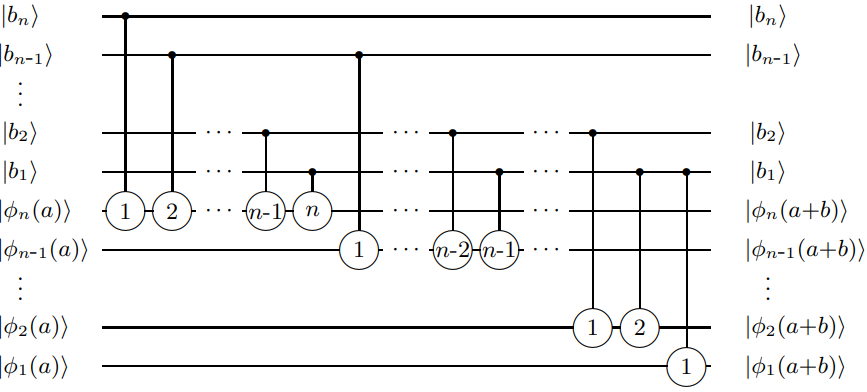
\includegraphics[width=\linewidth]{Quantum-Addition.PNG}
\centering
\end{figure}

Um die Addition in der Fourier-Basis zu realisieren,
wird kontrolliert eine Phasenverschiebung auf jedes Qubit des Quantenregister
\(\ket{\phi(a_n)}\) angewendet,
abhängig vom Inhalt des klassischen Registers \(\ket{b_n}\).
Dieses Vorgehen ermöglicht es,
die benötigten Qubits von \(3n\) auf \(n\) zu reduzieren.

Die in Abbildung~\ref{fig:Quantum-Addition} gezeigten Gatter werden durch ein klassisches Register kontrolliert,
um die Phasenverschiebung anzuwenden.
Da jedoch der klassische Wert im Voraus bekannt ist,
ist es möglich, die Phasenverschiebung, die auf die einzelnen Qubits angewendet wird,
im Voraus zu berechnen.
Dadurch wird die Anzahl der benötigten Phasen-Gatter auf dieselbe Anzahl an Qubits reduziert.
Dies führt zur Schaltung wie in Abbildung~\ref{fig:A_gate}.

\begin{figure}[!h]
\caption{Optimierte Quantum-Addition (vertauschte Bit-Reihenfolge)~\cite{beauregard2003circuit}}
\label{fig:A_gate}
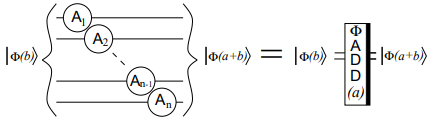
\includegraphics[width=\linewidth]{A_gate.PNG}
\centering
\end{figure}
Ein einzelnes Gatter aus Abbildung~\ref{fig:A_gate} realisiert dabei die folgende Transformation:

\begin{equation}
A_{x} = \prod_{k=1}^x{
\begin{pmatrix}
  1 & 0 \\
  0 & e^{({2\pi j})/({2^{k}})}
\end{pmatrix}^{(b_{x+1-k})}}
\end{equation}
Hier wird das Gatter \(A_{x}\) auf das Qubit \(x\) angewendet.
\(b_{x}\) repräsentiert die \(x\)-te Binärstelle des klassischen Summanden und
kann folglich die Werte \(0\) oder \(1\) annehmen.
Die Inverse des Adder-Gates realisiert die Subtraktion. 

\subsection{Modular-Adder-Gate}
Die Funktionalität der Schaltung besteht in der Berechnung von
\(\ket{(a+b) \bmod N}\).
Um dies zu gewährleisten, ohne dass das Quantenregister über- oder unterläuft,
wird das Register um ein sogenanntes "`Bedingung"'-Qubit erweitert.
Dieses Qubit wird mit \(\ket{0}\) initialisiert und
erweitert das Quantenregister \(\ket{B}\) als "`Most-Signifikant-Bit"'.
Zu Beginn addiert die Schaltung den klassischen Wert \(a\) auf das Quantenregister
\(\ket{B} = \phi(\ket{b} \otimes \ket{0})\).
Anschließend folgt die Anwendung eines inversen Adder-Gate,
das den klassischen Wert des Modulus \(N\) subtrahiert.
Dadurch ändert sich der Inhalt des Input-Quantenregister wie folgt:
\begin{equation*}
\ket{B} = \begin{cases}
  \ket{\phi(a+b-N)}             ,& \text{if } a+b \geq N,\\
  \ket{\phi(2^{n+1}-(N-(a+b)))} ,& \text{if } a+b < N
\end{cases}
\end{equation*}
Im ersten Fall der Gleichung befindet sich der Rest der Modulo Rechnung im Input-Quantenregister \(\ket{B}\).

Im zweiten Fall, befindet sich im Input-Quantenregister \(\ket{B}\) ein ungültiges Ergebnis.
Um die Berechnung umzukehren beziehungsweise zu korrigieren,
wird das "`Bedingung"'-Qubit genutzt.
Dieses hat durch die Berechnung den Zustand von \(\ket{0}\) auf \(\ket{1}\) gewechselt,
befindet sich jedoch noch immer in der Fourierbasis.
Nach der Anwendung der inversen Quanten-Fourier-Transformation
auf das Quantenregister \(\ket{B}\) wird das "`Bedingung"'-Qubit
mit einem kontrollierten NOT-Gate an ein zusätzliches Ancilla-Qubit mit dem Anfangszustand \(\ket{0}\) verbunden.

Abhängig vom Zustand des Ancilla Qubit wird mithilfe
eines kontrollierten Adder-Gates die Zahl \(N\) zum Quantenregister \(\ket{B}\) addiert.

Anschließend befindet sich unabhängig der beiden vorherigen Fälle,
der richtig berechnete Modulus im Quantenregister \(\ket{B}\).
Um zu vermeiden, dass für jedes Modular-Adder-Gate ein zusätzliches Ancilla-Qubit benötigt wird,
wird ein kontrollierter Bit-Flip auf dem Ancilla-Qubit durch das "`Bedingung"'-Qubit durchgeführt.
Dadurch wird das Ancilla-Qubit praktisch "`recycled"' und nimmt wieder den Anfangszustand \(\ket{0}\) an.
\begin{figure}[!h]
\caption{Modular-Adder-Gate~\cite{beauregard2003circuit}}
\label{fig:modular_adder_gate}
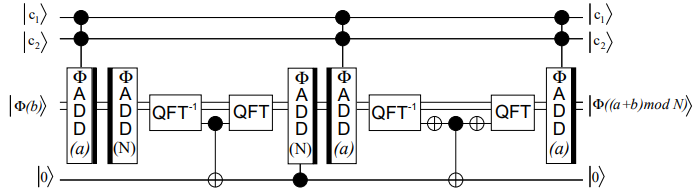
\includegraphics[width=\linewidth]{modular_adder_gate.PNG}
\centering
\end{figure}

\subsection{Controlled-Multiplier-Gate}
Das Controlled-Multiplier-Gate basiert hauptsächlich auf mehreren Modular-Adder-Gates,
wie in Abbildung~\ref{fig:modular_adder_gate} dargestellt.
Es verwendet ein einzelnes Modular-Adder-Gate,
um die Berechnung \(\ket{(x_i\cdot(2^ia)+b) \bmod N}\) durchzuführen,
wobei \(x_i\) das Qubit mit dem Index \(i\) in \(\ket{x}\) repräsentiert.

Das Gate ermöglicht die kontrollierte Multiplikation
eines Quantenregister \(\ket{X}\) mit dem klassischen Wert \(a\) und
die anschließende Addition eines Quantenregister \(\ket{B}\) im Wertebereich des Modulus \(N\).
Definiert man Quantenregister \(\ket{B}\) mit dem Inhalt \(\ket{b} = 0\),
erhält man die gewünschte Quantenschaltung zur Berechnung der gesuchten Funktionalität, den:
\(\ket{(a \cdot x) + 0\mod N} = \ket{(a \cdot x)\mod N}\).
Die Anwendung des Controlled-Multiplier-Gate als \(U_a\)-Gate wäre theoretisch möglich,
würde jedoch dazu führen, dass jedes verwendete \(U_a\)-Gate ein
zusätzliches \(n\)-Qubit-großes Quantenregister benötigt.
\begin{figure}[!h]
\caption{c-multiplier-gate~\cite{beauregard2003circuit}}
\label{fig:c-multiplier-gate}
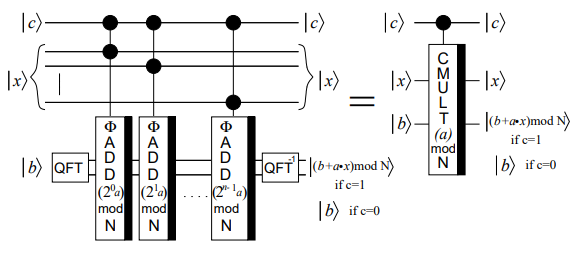
\includegraphics[width=\linewidth]{c-multiplier-gate.PNG}
\centering
\end{figure}

\subsection{Controlled-U-Gate}
Um das \(U_a\)-Gate ressourcenschonend zu implementieren,
wird das Controlled-Multiplier-Gate als Kernkomponente genutzt und um eine "`Recycling"'-Technik erweitert.

Der Aufbau besteht aus der Anwendung eines Controlled-Multiplier-Gates
mit dem Faktor \(a\) auf zwei Quantenregister \(\ket{X}\) und \(\ket{0}\).
Dadurch bleibt \(\ket{X}\) unverändert,
während das untere Register den Zustand von \(\ket{0}\) nach \(\ket{(a \cdot x) + 0\mod N}\) ändert.
Anschließend folgt ein Swap-Gate das die Qubits beider Quantenregister vertauscht.
Als letzten Schritt wird ein inverses Controlled-Multiplier-Gate
mit dem inversen Element von \(a\) also \(a^{-1} \bmod N\),
als Faktor angewendet.
Der Finale Zustand des oberen Quantenregisters beträgt nun \(\ket{(a \cdot x) \mod N}\),
während das untere Register sich im selben Zustand \(\ket{0}\) wie am Anfang befindet.

Das Element \(a^{-1} \bmod N\) kann klassisch
mit dem Erweiterter euklidischer Algorithmus berechnet werden.
Insgesamt werden für das \(U_a\)-Gate \(2n\) Qubits für die beiden Register benötigt,
einschließlich \(3\)~Qubits, wobei eines das Kontroll-Qubit des Gatters darstellt.
Die beiden anderen Qubits dienen als Ancilla- und "`Bedingungs"'-Qubit für die zugrunde liegenden Gatter.

Dadurch dass das untere Register des \(U_a\)-Gate den Zustand \(\ket{0}\) beibehält,
ist es möglich, mehrere \(U_a\)-Gate nacheinander auf den selben Registern anzuwenden.
Es werden also keine zusätzlichen Qubits in Abhängigkeit der Anzahl von \(U_a\)-Gatter benötigt. 

\begin{figure}[h]
\caption{Das Kontrollierte-\(U_a\) Gatter~\cite{beauregard2003circuit}}
\label{fig:c-Ugate}
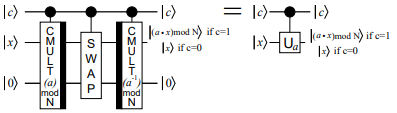
\includegraphics[width=\linewidth]{c-Ugate2.PNG}
\centering
\end{figure}

\subsection{Quantenschaltkreis Shor-Algortihmus}
Anschließend kann die Schaltung nach
Stêphane Beauregard~\cite{beauregard2003circuit} wie folgt aufgebaut werden:
\begin{figure}[!h]
\caption{Sequenzieller Shor-Algorithmus~\cite{beauregard2003circuit}}
\label{fig:Shor-Algorithmus}
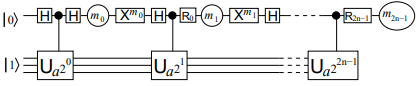
\includegraphics[width=\linewidth]{Shor-Algorithmus.PNG}
\centering
\end{figure}

Die Schaltung führt die Messung sowie die inverse Quanten-Fouriertransformation sequenziell durch.
Durch diese Methode wird der Gesamtbedarf auf \(2n+3\) Qubits reduziert,
im Vergleich zu \(4n+2\) Qubits,
die für die veraltete Variante von Qiskit benötigt würden~\cite{IBM:Shor_docu}.

\subsection{Primfaktorenbestimmung}
Nach der Durchführung des Quantenalgorithmus liefert die Messung des Quantenregisters \(\ket{X}\) die Phase \(P\),
die durch die Gleichung \(P = \frac{x}{2^{2n}}\) berechnet werden kann.
Anschließend wird der klassische Kettenbruchalgorithmus angewendet,
um einen Näherungsbruch zu erzeugen, bei dem die Periode \(r\) im Nenner steht.
Durch die Berechnung des größten gemeinsamen Teilers (greatest common divisor -- gcd)
können nun die beiden Primfaktoren ermittelt werden:
\(\gcd(a^{\frac{r}{2}}-1, N)\) und \(\gcd(a^{\frac{r}{2}}+1, N)\).

Es ist möglich, dass nur einer oder kein Faktor gefunden wird,
da der Shor-Algorithmus ein probabilistischer Algorithmus ist und
deswegen keine deterministischen Ergebnisse garantiert.
Wenn nur ein Faktor \(F\) gefunden wird,
kann der zweite Faktor logischerweise durch \(\frac{N}{F}\) berechnet werden.
Wenn kein Faktor gefunden wurde, wird der gesamte Shor-Algorithmus erneut durchgeführt.
Es kann sinnvoll sein, nach mehreren erfolglosen Versuchen ein anderes \(a\) auszuwählen.~\cite{Mounica}

Die Nachbearbeitung des Shor-Algorithmus umfasst also die Auswertung der gemessenen Phasen,
die Anwendung des Kettenbruchalgorithmus zur Ermittlung der Periode und
schließlich die Berechnung der Primfaktoren mithilfe des größten gemeinsamen Teilers.

\section{Beispiel Qiskit}
Die Implementierung der \(U_a\)-Gatter entspricht dem Aufbau von
Stêphane Beauregard~\cite{beauregard2003circuit},
wie im vorherigen Abschnitt beschrieben.
Allerdings wird in der Implementierung die Reihenfolge
der sequentiellen inverse-Quanten-Fouriertransformation und
die Reihenfolge der \(U_a\)-Gatter in gespiegelter Reihenfolge angewendet.

Die Quanten-Fouriertransformation nach
Stêphane Beauregard~\cite{beauregard2003circuit} behält
nach der Anwendung die Reihenfolge der Qubits bei.
Diese Version der Quanten-Fouriertransformation stimmt nicht
mit anderen Literaturquellen überein.
Normalerweise ist die Reihenfolge der Qubits
nach der Quanten-Fouriertransformation umgekehrt~\cite{Hoever:QC,Young:QFT} oder
es werden Swap-Gates verwendet,
um die ursprüngliche Reihenfolge wiederherzustellen~\cite{IBM:QFT}.

\subsection{Shor-Algorithmus für \(N = 21\)}
Im Folgenden wird der Shor-Algorithmus verwendet,
um die Zahl \(N = 21\) zu faktorisieren.
Der Quantencomputer, der für die Ausführung des Algorithmus benötigt wird,
wird mithilfe des Qiskit-Simulators simuliert.
Es wird keine größere Zahl als \(21\) simuliert
da ansonsten die Schaltkreisgrafiken nicht mehr lesbar wären und
die Simulation ab einer Zahl \(N > 256\) zu viel Zeit in Anspruch nehmen würde.

In Abbildung~\ref{fig:QiskitN1a17} sieht man den Aufbau des Quantenschaltkreises
für die Wahl von \(a = 17\).
Bei wiederholter Ausführung des Algorithmus wird deutlich,
dass dieser probabilistischer Natur ist.
In Abbildung~\ref{fig:shor_countsN21a17} sind die Messergebnisse dargestellt,
die trotz gleichbleibender Parameter unterschiedlich sind.
Es wird auch deutlich, dass der Algorithmus nur probabilistisch ein korrektes Ergebnis liefert.
Wählt man beispielsweise von den beiden häufigsten Messergebnis die "`0000 0000"',
würde man keinen der beiden Primfaktoren erhalten.
Mit der Zahl "`1000 0000"', die  genau so oft gemessen wurde, könnte man die Primfaktoren bestimmen:
\begin{equation*}
\begin{split}
  N = 21,
  n = 5,
  a = 17\,10\,0000\,0000_2 \eqq 512_{10}\\
  512/2^{2\cdot n} = 0.5\\
  \fraction(0.5) = \frac{1}{2}
\end{split}
\end{equation*}
In diesem Fall wäre die Berechnung eines Näherungsbruchs mit dem Kettenbruchalgorithmus nicht nötig gewesen.
Die Berechnung wird mit dem Nenner fortgesetzt:
\begin{equation*}
\begin{split}
  \gcd(a**(2//2)-1, N) = 1\\
  \gcd(a**(2//2)+1, N) = 3
\end{split}
\end{equation*}
Für dieses Messergebnis konnte mit der klassischen Nachberechnung
nur einer der beiden Primaktoren gefunden werden.
Logischerweise kann in diesem Fall der andere Primfaktor mit einer einfachen Division berechnet werden:
\(\frac{N}{3} = 7\).

\subsection{Vereinfachungen Shor-Algorithmus}
In Abbildung~\ref{fig:QiskitN1a13} sieht man,
dass die Wahl der Zahl \(a\) erheblichen Einfluss auf die Komplexität der \(U_a\)-Gatter der Schaltung hat.
Anhand der zugehörigen Messung in Abbildung~\ref{fig:shor_countsN21a13} wird deutlich,
dass das wechseln der Zahl \(a\) nach mehreren Fehlversuchen sinnvoll sein kann.

\section{Ausblick}
Im weiteren Verlauf dieser Arbeit wird die vorhandene Implementierung des Shor-Algorithmus
als Teil der Bibliothek genutzt,
um einen Algorithmus zu entwerfen, der in der Lage ist,
den privaten Schlüssel des RSA-Verfahrens aus den öffentlichen Schlüsseln zu berechnen.

Desweiteren spielt der Grover-Algorithmus eine wichtige Rolle für die Kryptoanalyse mit Quantencomputern,
weswegen dieser auch Einzug in die Bibliothek finden wird.

In zukünftigen Arbeiten könnten die Algorithmen weiter vertieft werden,
was jedoch fortgeschrittenes Wissen im Bereich des Quantencomputings erfordert.
Dabei könnte man sich zum Beispiel damit beschäftigen,
ob Vereinfachungen des Shor-Algorithmus möglich sind, falls man ein \(a\) wählt,
welches die Gatter der Schaltung in einem Vergleichbaren Zustand wie Abbildung~\ref{fig:QiskitN1a17} bringt.

Zukünftig wird die Fehlerkorrektur eine wichtige Rolle spielen.
Im Bezug dazu könnte man sich mit Möglichkeiten zur Fehlerminimierung oder Fehlerkorrektur auseinandersetzen.
Man könnte zum Beispiel Untersuchen, wie es sich Auswirkt,
wenn die vollständige Quanten-Fouriertransformation durch eine approximative Variante ersetzt wird.

\begin{figure*}[p]
\centering
\caption{Sequenzieller Shor-Algorithmus Qiskit N=21, a=17}
\label{fig:QiskitN1a17}
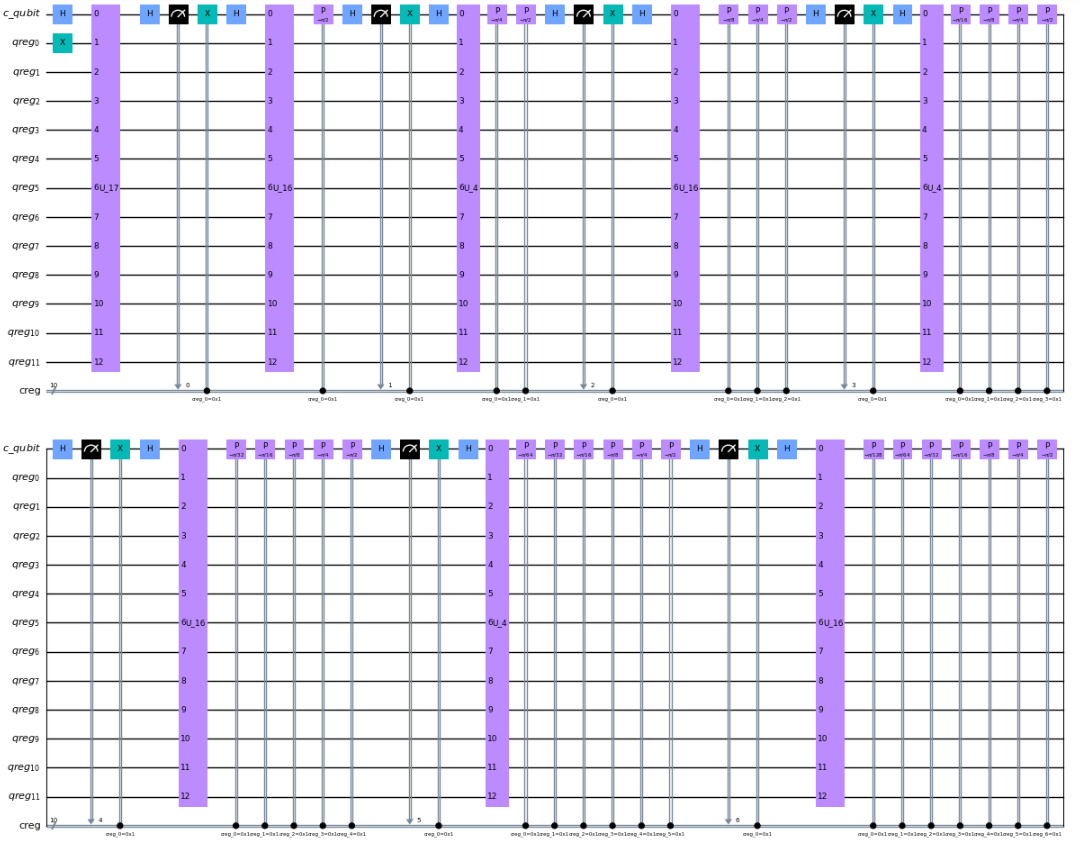
\includegraphics[height=\linewidth,angle=90]{qiskit_Shor_21_a17.PNG}
\end{figure*}

\begin{figure*}[p]
\centering
\caption{Sequenzieller Shor-Algorithmus Qiskit N=21, a=13}
\label{fig:QiskitN1a13}
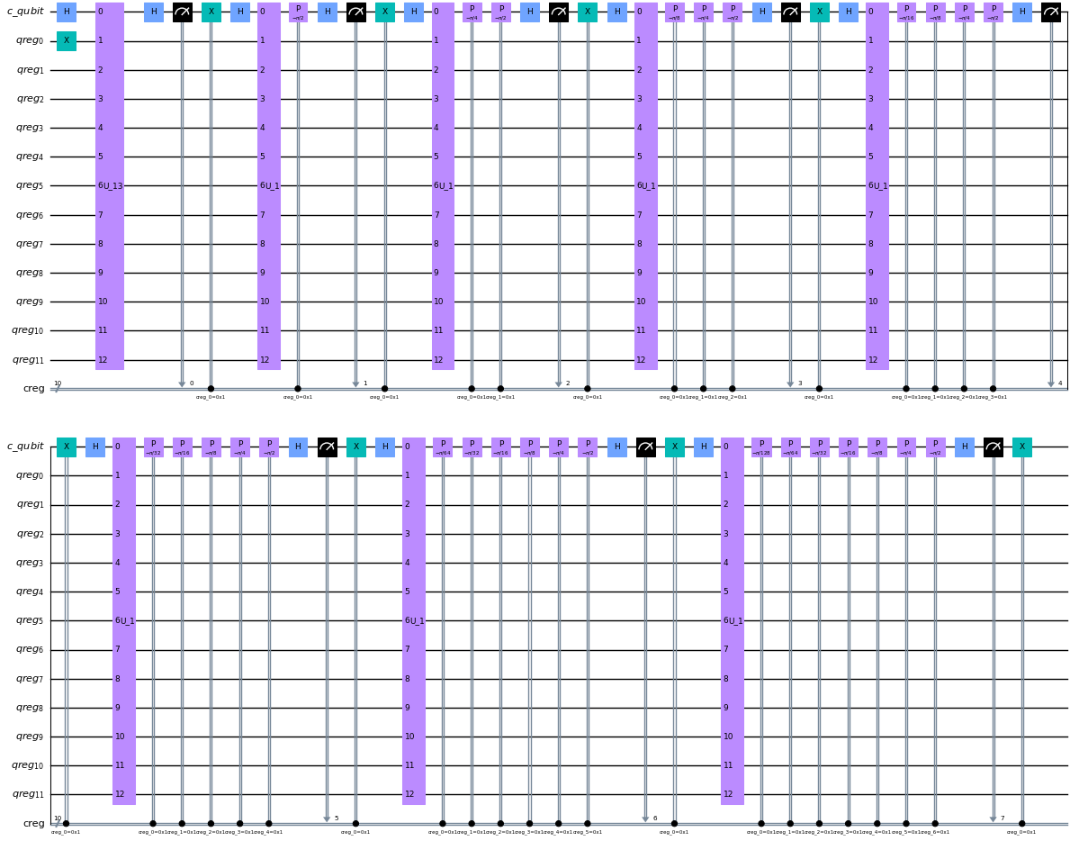
\includegraphics[height=\linewidth,angle=90]{qiskit_Shor_21_a13.PNG}
\end{figure*}

\clearpage
\begin{figure}[p]
\caption{Messung sequenzieller Shor-Algorithmus Qiskit N=21, a=17}
\label{fig:shor_countsN21a17}
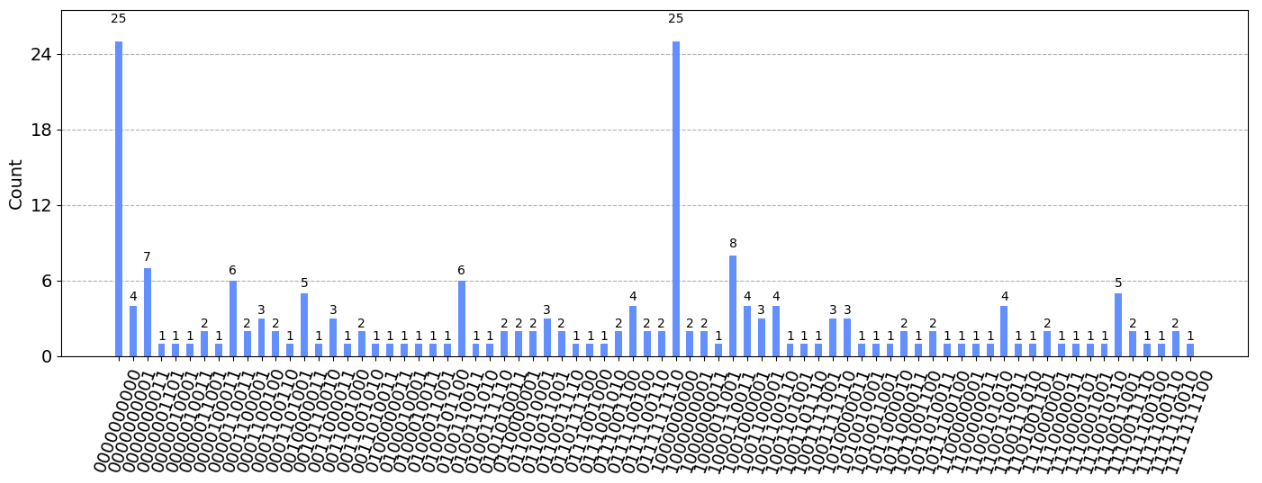
\includegraphics[height=\linewidth,angle=90]{shor_countsN21a17.PNG}
\end{figure}
\begin{figure}[p]
\caption{Messung sequenzieller Shor-Algorithmus Qiskit N=21, a=13}
\label{fig:shor_countsN21a13}
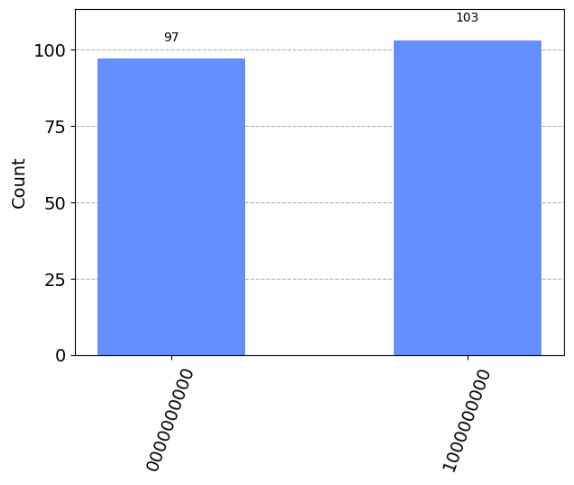
\includegraphics[height=\linewidth,angle=90]{shor_countsN21a13.PNG}
\end{figure}
\clearpage

\bibliography{IEEEabrv,sample}

\end{document}
